\documentclass{article}

\usepackage{arxiv}
\usepackage[utf8]{inputenc}
\usepackage[T1]{fontenc}
\usepackage{mathptmx}
\usepackage{amsmath,amssymb,amsthm}
\usepackage{bm}
\usepackage{url}
\usepackage{booktabs}
\usepackage{tabularx}
\usepackage{graphicx}
\usepackage{microtype}
\usepackage[authoryear,round]{natbib}
\usepackage{xcolor}
\usepackage{enumitem}
\usepackage{algorithm}
\usepackage[noend]{algpseudocode}
\usepackage{tikz}
\usetikzlibrary{positioning,fit,backgrounds,calc,arrows.meta}
\usepackage[font=small,labelfont=bf,labelsep=period]{caption}

\definecolor{OIblue}{HTML}{0072B2}
\definecolor{OIgreen}{HTML}{009E73}
\definecolor{linkblue}{HTML}{1F4E79}
\usepackage{hyperref}
\hypersetup{colorlinks=true, linkcolor=linkblue, citecolor=linkblue, urlcolor=linkblue,
  pdftitle={Words to Coordinates: An Uncertainty-Aware NLP-Geospatial Framework for Measuring the Gap Between Disclosed and Physical Climate Risk},
  pdfauthor={Thanatchon Chongmankhong},
  pdfkeywords={climate risk disclosure, physical climate risk, natural language processing, geospatial analysis, uncertainty quantification, sustainable finance}}

\theoremstyle{plain}
\newtheorem{proposition}{Proposition}
\newtheorem{corollary}{Corollary}
\theoremstyle{definition}
\newtheorem{definition}{Definition}
\newtheorem{remark}{Remark}

\algrenewcommand\algorithmicrequire{\textbf{Input:}}
\algrenewcommand\algorithmicensure{\textbf{Output:}}
\setlist{itemsep=2pt, topsep=3pt}
\raggedbottom
\makeatletter
\setlength{\@fptop}{0pt}
\setlength{\@fpbot}{0pt plus 1fil}
\makeatother

\newcommand{\DGI}{\mathrm{DGI}}
\newcommand{\x}{\mathbf{x}}
\newcommand{\E}{\mathbb{E}}

\renewcommand{\shorttitle}{Words to Coordinates}

\title{Words to Coordinates: An Uncertainty-Aware NLP--Geospatial Framework for Measuring the Gap Between Disclosed and Physical Climate Risk}

\author{Thanatchon Chongmankhong}

\date{November 2026}

\begin{document}
\maketitle

\begin{abstract}
Corporate climate disclosure is being standardised rapidly, with IFRS~S2 emerging as a global baseline, yet the information that matters most for physical climate risk---where a firm's assets are and which hazards they face---remains embedded in unstructured, multilingual reports. Text-based measures of firm climate exposure capture what firms say but not what their assets face, while geospatial assessments rely on curated asset databases and ignore disclosure content. We propose \emph{Words to Coordinates} (W2C), a framework that links the two. W2C extracts taxonomy-aligned climate disclosures and asset locations from reports with page-level provenance, resolves assets to coordinates, overlays them with scenario-based hazard projections, and compares modelled exposure with disclosed risk through a Disclosure Gap Index that places firms in four quadrants: aware, silent risk, cheap talk and benign. Two design choices distinguish W2C: distant supervision from XBRL-tagged filings, to extend coverage to under-served and non-English markets, and end-to-end propagation of extraction, geolocation and hazard-model uncertainty, so that every classification carries a calibrated probability. We derive a closed-form relation between geolocation error and the fidelity of exposure estimates, which implies that location error should not exceed one third of a hazard's spatial correlation length. A simulation study on the real locations of 11,107 power plants held by 1,247 owners in 76 countries confirms the relation (mean absolute deviation 0.002) and shows that (i)~country-level geocoding preserves a firm-level rank correlation of at most 0.54, even for spatially coherent hazards; (ii)~for local hazards, city-level geolocation error degrades quadrant classification more than five times as much as a 20\% extraction error rate; and (iii)~full uncertainty propagation reduces expected calibration error from 0.075 to 0.033 and supports selective identification of silent-risk firms at 84\% precision. We close with an evaluation protocol and identification strategies for a global empirical application.
\end{abstract}

\keywords{Climate risk disclosure \and Physical climate risk \and Natural language processing \and Geospatial analysis \and Uncertainty quantification \and Sustainable finance}

% =====================================================================
\section{Introduction}
\label{sec:intro}

Climate-related financial disclosure is moving from voluntary frameworks to mandatory, standardised reporting. Building on the recommendations of the Task Force on Climate-related Financial Disclosures \citep{tcfd2017}, the International Sustainability Standards Board (ISSB) issued IFRS~S1 and IFRS~S2 in June 2023, effective for annual reporting periods beginning on or after 1 January 2024 \citep{ifrs2023s1,ifrs2023s2}. A growing number of jurisdictions are adopting or adapting these standards, alongside the European Sustainability Reporting Standards (ESRS) \citep{ec2023esrs}. Institutional investors report that climate risks matter for their decisions \citep{krueger2020importance}, yet the data on which those decisions rest are contested: ESG ratings from different providers diverge substantially \citep{berg2022aggregate}, and so do commercial metrics of physical climate risk \citep{hain2022physical}.

Two research traditions measure firm-level climate risk from different raw material. The first is textual. Climate exposure has been measured from earnings-call transcripts \citep{sautner2023firm}, and domain-adapted language models such as ClimateBERT \citep{webersinke2021climatebert} have been used to classify climate disclosures, detect environmental claims and quantify the specificity of corporate commitments \citep{bingler2022cheap,stammbach2023environmental,schimanski2024bridging}. Large language models now support question answering over sustainability reports \citep{ni2023chatreport} and are evaluated on retrieval benchmarks built from corporate climate disclosures \citep{schimanski2024climretrieve}. These measures capture what firms \emph{say}, but not what their physical assets \emph{face}. The second tradition is geospatial. Spatial finance overlays the locations of physical assets with hazard data to estimate exposure from the bottom up \citep{caldecott2022spatial}, using projections derived from climate model ensembles \citep{eyring2016cmip6,thrasher2022nex} and hazard maps such as Aqueduct \citep{ward2020aqueduct,kuzma2023aqueduct}. These measures capture what assets face, but they rely on curated asset databases that cover a limited set of sectors and markets, and they are silent about what firms disclose.

The question that connects the two traditions is, in our view, among the most policy-relevant in sustainable finance: \emph{do firms disclose the physical climate risks to which their assets are actually exposed, and where are the gaps largest?} Supervisors need the answer to target reviews, investors to price undisclosed risk, and assurance providers to test the completeness of disclosures. Answering it requires linking words to coordinates at scale: extracting both disclosure content and asset locations from the same documents, across languages and reporting regimes, with traceable provenance and quantified uncertainty. Coverage compounds the difficulty. ESG data are concentrated on large firms in developed markets \citep{kotsantonis2019four}, leaving \emph{ESG data deserts} in emerging markets, where physical hazards are often severe and disclosures appear in local languages and unstructured formats.

This paper makes four contributions.
\begin{enumerate}[leftmargin=1.6em]
  \item \textbf{Measurement.} We formalise the \emph{Disclosure Gap Index} (DGI), which compares a firm's modelled physical exposure with its disclosure intensity within a peer group, and the \emph{disclosure--exposure plane}, which classifies firms as aware, silent risk, cheap talk or benign (Section~\ref{sec:problem}).
  \item \textbf{Framework.} We specify Words to Coordinates (W2C), an end-to-end architecture that is provenance-first (every extracted value is linked to a document, page and bounding box), taxonomy-aligned (an IFRS~S2 schema with crosswalks to ESRS~E1 and GRI~305) and coverage-oriented, using XBRL-tagged filings as distant supervision for multilingual extraction (Section~\ref{sec:framework}).
  \item \textbf{Theory.} We derive a closed-form relation between geolocation error and the correlation between true and estimated hazard exposure. It yields a simple design rule---location error should not exceed one third of the hazard's spatial correlation length---that tells a pipeline how precise its geocoding must be for each hazard (Section~\ref{sec:precision}).
  \item \textbf{Evidence on measurement properties.} A simulation study grounded in the real locations of 11,107 power plants confirms the theory, quantifies how extraction and geolocation errors combine in quadrant classification, and shows that end-to-end uncertainty propagation yields calibrated probabilities that support selective identification of silent-risk firms (Section~\ref{sec:sim}).
\end{enumerate}

\paragraph{Scope.} This is a framework and methods paper. It does not report disclosure gaps for real firms: the disclosure variables and hazard fields in our simulation are synthetic, and only the asset geography is real. We instead establish the measurement properties of the DGI under controlled conditions in which the ground truth is known, and set out the evaluation protocol (Section~\ref{sec:eval}) and identification strategies (Section~\ref{sec:agenda}) for the empirical programme that the framework is designed to support. Section~\ref{sec:discussion} discusses limitations and ethical considerations, and Section~\ref{sec:conclusion} concludes.

% =====================================================================
\section{Related work}
\label{sec:related}

\paragraph{NLP for climate and ESG disclosure.} Early work established datasets for detecting climate-related text \citep{varini2020climatext} and verifying climate claims \citep{diggelmann2020climatefever}, and applied NLP to sustainability reports \citep{luccioni2020analyzing}. ClimateBERT \citep{webersinke2021climatebert} enabled analyses showing that much corporate climate disclosure is non-specific ``cheap talk'' \citep{bingler2022cheap} and that regulatory disclosure of transition and physical risks is reflected in credit default swap spreads \citep{kolbel2024askbert}. Subsequent work extended measurement to environmental claims \citep{stammbach2023environmental} and to ESG communication more broadly \citep{schimanski2024bridging}, and used retrieval-augmented generation \citep{lewis2020rag} for report analysis \citep{ni2023chatreport,schimanski2024climretrieve}. Two gaps motivate W2C. First, these systems output labels or answers rather than structured, taxonomy-aligned values with provenance and calibrated uncertainty. Second, they rarely extract the geographic information---sites, facilities and locations---that would allow disclosures to be checked against physical exposure.

\paragraph{Physical climate risk and spatial finance.} Physical risk assessment combines hazard, exposure and vulnerability. Hazard projections derive from CMIP6 ensembles \citep{eyring2016cmip6} under ScenarioMIP pathways \citep{oneill2016scenariomip}, often statistically downscaled \citep{thrasher2022nex}; specialised products cover floods and water stress \citep{ward2020aqueduct,kuzma2023aqueduct}, tropical cyclones \citep{knapp2010ibtracs} and supervisory scenarios \citep{ngfs2023}. Spatial finance links such hazard data to asset-level datasets \citep{caldecott2022spatial}, including open registries of power plants \citep{byers2018gppd}, energy infrastructure \citep{gem2024} and emission sources \citep{climatetrace2024}. \citet{hain2022physical} show that physical risk scores from different providers disagree substantially. Text-based measures \citep{sautner2023firm} sidestep the need for locations, but measure attention to climate topics rather than exposure. W2C treats location as an uncertain, extracted quantity and propagates its uncertainty.

\paragraph{Disclosure standards as an extraction target.} IFRS~S2 requires disclosure of climate-related risks and opportunities (\P\,10), of climate resilience assessed with scenario analysis (\P\,22), of cross-industry metrics including Scope~1--3 greenhouse gas emissions and the amount and percentage of assets or business activities vulnerable to physical risks (\P\,29), and of climate-related targets (\P\P\,33--36) \citep{ifrs2023s2}. ESRS~E1 \citep{ec2023esrs} and GRI~305 \citep{gri305} contain overlapping requirements, and the TNFD recommendations make location the explicit first step of nature-related assessment \citep{tnfd2023}. Standardisation turns disclosures into a well-defined extraction target, and digital taxonomies with XBRL tagging, where they exist, provide machine-readable labels that W2C exploits as distant supervision.

\paragraph{Distant supervision, calibration and uncertainty.} Distant supervision aligns an existing knowledge base with text to create noisy training labels \citep{mintz2009distant}, and knowledge distillation transfers the behaviour of a large model to a smaller one \citep{hinton2015distilling}. Probabilistic predictions should be calibrated \citep{guo2017calibration} and evaluated with proper scoring rules \citep{brier1950}; conformal prediction provides distribution-free coverage guarantees for set-valued outputs \citep{vovk2005algorithmic,angelopoulos2023gentle}, and selective classification formalises abstention \citep{geifman2017selective}. Measurement error in explanatory variables biases downstream estimates \citep{carroll2006measurement}, which is why W2C carries uncertainty through to its outputs rather than discarding it after extraction.

% =====================================================================
\section{Problem formulation}
\label{sec:problem}

\subsection{Setup}
Consider a set of firms $\mathcal{I}$ in a comparison set, for example a sector--year. Firm $i$ controls assets $a\in\mathcal{A}_i$ with locations $\x_a$ on the sphere and non-negative weights $w_a$, $\sum_{a\in\mathcal{A}_i} w_a = 1$, that reflect the share of capacity, asset value or revenue attributable to each asset. Physical hazards $h\in\mathcal{H}$ (riverine and coastal flooding, extreme heat, drought, tropical cyclones, wildfire) are described by hazard fields $Z_{h,s,t}(\x)$ under scenario $s$ and time horizon $t$, available as an ensemble $\{Z^{(m)}_{h,s,t}\}_{m=1}^{M}$ of model outputs. We suppress $h,s,t$ when unambiguous.

\begin{definition}[Modelled exposure]
The modelled exposure of firm $i$ is
\begin{equation}
  E_i = \sum_{a\in\mathcal{A}_i} w_a\, g\big(Z(\x_a)\big),
  \label{eq:exposure}
\end{equation}
where $g$ is a monotone transform mapping hazard intensity to a normalised exposure or damage score.
\end{definition}

\begin{definition}[Disclosure intensity]
For each hazard, the disclosure intensity $D_i\in\{0,\dots,4\}$ of firm $i$ is an ordinal level:
\begin{enumerate}[label=\arabic*., start=0, leftmargin=1.8em]
  \item \emph{None}: no reference to the physical risk;
  \item \emph{Generic}: physical climate risk mentioned without hazard specificity;
  \item \emph{Hazard-specific}: the hazard is identified and linked to operations or locations;
  \item \emph{Quantified}: exposure or anticipated financial effects are quantified (cf.\ IFRS~S2 \P\,29(c));
  \item \emph{Quantified with scenarios and adaptation}: quantified effects under named scenarios, with a resilience or adaptation response (cf.\ IFRS~S2 \P\,22).
\end{enumerate}
\end{definition}

The scale is hazard-specific: a firm may disclose flood risk at level~3 and heat risk at level~0.

\begin{definition}[Disclosure Gap Index]
Let $F_E$ and $F_D$ denote the mid-rank empirical distribution functions of $E$ and $D$ within the comparison set. The Disclosure Gap Index of firm $i$ is
\begin{equation}
  \DGI_i = F_E(E_i) - F_D(D_i) \in (-1, 1).
  \label{eq:dgi}
\end{equation}
\end{definition}

Positive values indicate disclosure below what the firm's relative exposure would suggest; negative values indicate disclosure beyond it. Because both terms are peer-relative, the DGI is invariant to monotone transformations of $E$ and comparable across hazards and sectors.

\begin{definition}[Disclosure--exposure quadrants]
Given thresholds $\tau_E\in(0,1)$ and $\tau_D\in\{1,\dots,4\}$, firm $i$ is classified as
\begin{equation}
  Q_i =
  \begin{cases}
    \text{aware} & \text{if } F_E(E_i) > \tau_E \text{ and } D_i \geq \tau_D,\\
    \text{silent risk} & \text{if } F_E(E_i) > \tau_E \text{ and } D_i < \tau_D,\\
    \text{cheap talk} & \text{if } F_E(E_i) \leq \tau_E \text{ and } D_i \geq \tau_D,\\
    \text{benign} & \text{otherwise.}
  \end{cases}
  \label{eq:quadrant}
\end{equation}
\end{definition}

We use $\tau_E = 0.5$ and $\tau_D = 2$ throughout, so that \emph{silent risk} denotes an above-median exposed firm that discloses no hazard-specific information. Figure~\ref{fig:plane} illustrates the plane. We borrow the term \emph{cheap talk} from \citet{bingler2022cheap} to denote disclosure intensity that exceeds modelled exposure; the label is descriptive rather than normative, because such disclosure may reflect exposures outside the hazard model, such as supply-chain risks, or prudent reporting.

\begin{figure}[t]
  \centering
  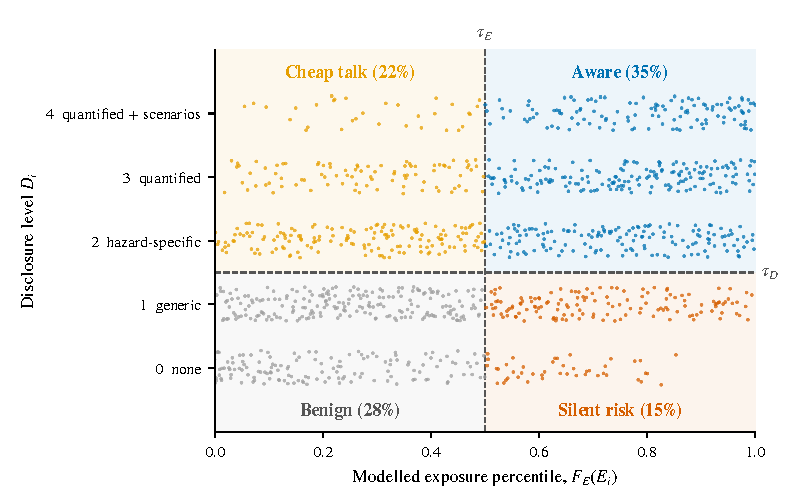
\includegraphics{figs/fig_de_plane.pdf}
  \caption{The disclosure--exposure plane for one simulated replicate (1,247 firms; real asset locations, synthetic hazard with $\ell = 50$~km and synthetic disclosures). Points are jittered vertically. Dashed lines mark the thresholds $\tau_E = 0.5$ and $\tau_D = 2$; percentages give the share of firms in each quadrant.}
  \label{fig:plane}
\end{figure}

\subsection{Uncertainty and probabilistic classification}
\label{sec:uncertainty}

None of the inputs to \eqref{eq:exposure}--\eqref{eq:quadrant} is observed without error. A pipeline observes (i)~an extracted level $\hat D_i$ with a calibrated predictive distribution $P(D_i \mid \hat D_i)$; (ii)~estimated locations $\hat\x_a$ with a precision class $r(a)$ and an error scale $\sigma_{r(a)}$; and (iii)~an ensemble of hazard models rather than the hazard itself. We therefore treat $\DGI_i$ and $Q_i$ as random variables and report $P(Q_i = q \mid \text{data})$ together with quantiles of $\DGI_i$, computed by Monte Carlo (Algorithm~\ref{alg:mc}). Because exposure enters through peer-relative ranks, the classification of one firm depends on the uncertain exposures of all firms; the Monte Carlo therefore recomputes ranks in every draw. A firm is flagged as silent risk only if $P(Q_i = \text{silent risk}) \geq \tau_p$; otherwise the pipeline abstains, which is a selective classification rule \citep{geifman2017selective}.

\subsection{How precise must geolocation be?}
\label{sec:precision}

Geolocation is the step most often skipped or approximated: firms are frequently assigned to the country or city of their headquarters. The precision required depends on the hazard. Model a hazard locally as a stationary Gaussian random field with unit variance and squared-exponential correlation $\rho(d) = \exp\{-d^2/(2\ell^2)\}$, where $\ell$ is the correlation length, and model geolocation error as isotropic Gaussian, $\hat\x = \x + \bm\delta$ with $\bm\delta\sim\mathcal{N}(\mathbf{0}, \sigma^2 I_2)$ independent of the field.

\begin{proposition}
\label{prop:corr}
Under these assumptions,
\begin{equation}
  \operatorname{Corr}\big(Z(\x), Z(\hat\x)\big) = \frac{\ell^2}{\ell^2 + \sigma^2}.
  \label{eq:pearson}
\end{equation}
Moreover, for any strictly increasing $g$, the Spearman correlation between $g(Z(\x_a))$ and $g(Z(\hat\x_a))$ across assets that are mutually independent (separated by distances large relative to $\ell$) is
\begin{equation}
  \rho_S(\sigma/\ell) = \frac{6}{\pi}\int_0^\infty \arcsin\!\Big(\tfrac{1}{2}\,e^{-(\sigma/\ell)^2 t}\Big)\, e^{-t}\, dt .
  \label{eq:spearman}
\end{equation}
Both quantities depend on $\sigma$ and $\ell$ only through the ratio $\sigma/\ell$.
\end{proposition}

The proof is given in Appendix~\ref{app:proof}. Inverting \eqref{eq:pearson} gives a design rule.

\begin{corollary}[Design rule]
\label{cor:rule}
$\operatorname{Corr}(Z(\x), Z(\hat\x)) \geq \rho^\ast$ if and only if $\sigma \leq \ell\sqrt{1/\rho^\ast - 1}$. In particular, preserving a correlation of $0.9$ requires $\sigma \leq \ell/3$.
\end{corollary}

The rule turns an abstract accuracy target into a per-hazard engineering specification. As a stylised guide, hazards such as riverine flooding vary over distances of a few kilometres, whereas heat extremes are typically coherent over hundreds of kilometres; the corresponding precision requirements differ by two orders of magnitude. Figure~\ref{fig:thailand} illustrates the intuition with real plant locations in Thailand.

\begin{figure}[t]
  \centering
  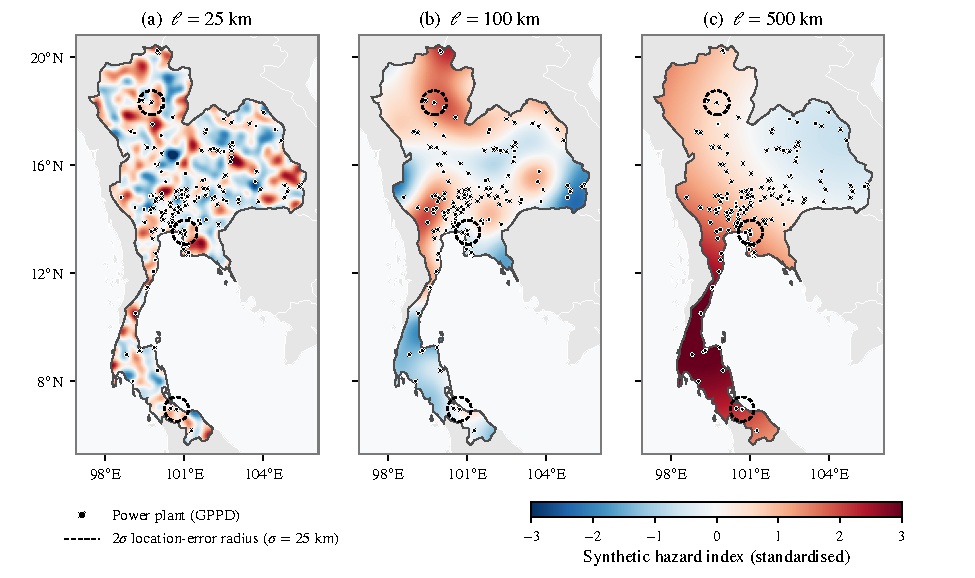
\includegraphics{figs/fig_thailand.pdf}
  \caption{The same synthetic hazard pattern rendered at three correlation lengths over Thailand, with the 196 Thai plants in the Global Power Plant Database \citep{byers2018gppd}. Dashed circles show a $2\sigma$ radius for city-level geolocation error ($\sigma = 25$~km) around three large plants. For a local hazard (a), the circle spans several independent hazard features, so an exposure estimate from the wrong location is close to a random draw; for a regional hazard (c), the hazard is nearly constant within the circle. The fields are synthetic and do not represent actual hazards in Thailand.}
  \label{fig:thailand}
\end{figure}

\begin{remark}[Finite domain]
\label{rem:finite}
Proposition~\ref{prop:corr} describes independent assets. When assets are clustered relative to $\ell$, correlations computed within a single sample fall slightly below \eqref{eq:pearson}, because the sample variance of exposure shrinks. With $\bar c$ the mean pairwise correlation $\rho(d_{ab})$ among assets, the within-sample analogue of \eqref{eq:pearson} is approximately $(\rho - \bar c)/(1 - \bar c)$, where $\rho = \ell^2/(\ell^2+\sigma^2)$ (Appendix~\ref{app:proof}).
\end{remark}

% =====================================================================
\section{The Words to Coordinates framework}
\label{sec:framework}

Figure~\ref{fig:arch} summarises the architecture. Its organising idea is that disclosure (what firms say) and exposure (what assets face) are extracted from the same documents but processed in two lanes with different error models, and are reconciled only at the end, through the Monte Carlo step that produces the DGI and quadrant probabilities.

\begin{figure}[t]
  \centering
  \begin{tikzpicture}[
  font=\sffamily\scriptsize,
  >={Stealth[length=4.2pt,width=3.4pt]},
  base/.style={draw, rounded corners=2pt, align=center, inner sep=3.2pt, line width=0.45pt},
  neutral/.style={base, draw=black!45, fill=black!4},
  tl/.style={base, draw=OIblue!85!black, fill=OIblue!7, text width=6.75cm, minimum height=1.02cm},
  gl/.style={base, draw=OIgreen!85!black, fill=OIgreen!8, text width=6.75cm, minimum height=1.02cm},
  outp/.style={base, draw=black!45, fill=white, text width=4.55cm, minimum height=1.0cm},
  hdr/.style={align=center, font=\sffamily\scriptsize\bfseries},
  arr/.style={->, line width=0.55pt, draw=black!70},
]
% ---- shared upstream stages
\node[neutral, text width=15.25cm] (src) at (0,0)
  {\textbf{Disclosure sources}\\[1pt]
   SEC EDGAR \textperiodcentered{} EDINET \textperiodcentered{} DART \textperiodcentered{}
   SET Form 56-1 One Report \textperiodcentered{} ESEF \textperiodcentered{} BRSR (XBRL)\\
   sustainability, TCFD and ISSB reports (PDF, many languages)};
\node[neutral, text width=15.25cm, below=4.5mm of src] (doc)
  {\textbf{Document AI with provenance}\\[1pt]
   layout parsing, OCR, table and chart extraction; every element keyed by
   (document hash, page, bounding box)};

% ---- text lane
\node[hdr, text=OIblue!85!black] (th) at (-3.95,-2.62) {Text lane: what firms disclose ($\hat D$)};
\node[tl, below=2.2mm of th] (t1)
  {\textbf{Hybrid retrieval}\\[1pt] BM25 + multilingual dense embeddings\\ + visual page retrieval};
\node[tl, below=4.2mm of t1] (t2)
  {\textbf{Taxonomy-aligned extraction}\\[1pt] IFRS S2 schema with crosswalks to ESRS E1 and GRI 305;\\
   student model trained by XBRL distant supervision};
\node[tl, below=4.2mm of t2] (t3)
  {\textbf{Verification and calibration}\\[1pt] unit normalisation, consistency checks,\\
   calibrated $P(D\mid\hat D)$ and conformal prediction sets};

% ---- geo lane
\node[hdr, text=OIgreen!80!black] (gh) at (3.95,-2.62) {Geo lane: what assets face ($\hat E$)};
\node[gl, below=2.2mm of gh] (g1)
  {\textbf{Entity and asset resolution}\\[1pt] LEI and parent links; asset registries
   (GEM, Climate TRACE, GPPD, OSM)};
\node[gl, below=4.2mm of g1] (g2)
  {\textbf{Geocoding with precision classes}\\[1pt] coordinates $\hat{\mathbf{x}}_a$ with error scale
   $\sigma_r$, from site to country level};
\node[gl, below=4.2mm of g2] (g3)
  {\textbf{Hazard overlay}\\[1pt] CMIP6, Aqueduct, IBTrACS $\times$ SSP scenario $\times$ horizon;\\
   multi-model ensemble $\{Z^{(m)}\}$};

\begin{scope}[on background layer]
  \node[draw=OIblue!70, dashed, rounded corners=3pt, line width=0.5pt, fill=OIblue!2,
        inner sep=2.6mm, fit=(th)(t1)(t2)(t3)] (tbox) {};
  \node[draw=OIgreen!70, dashed, rounded corners=3pt, line width=0.5pt, fill=OIgreen!2,
        inner sep=2.6mm, fit=(gh)(g1)(g2)(g3)] (gbox) {};
\end{scope}

\draw[arr] (src) -- (doc);
\draw[arr] (doc.south -| tbox.north) -- (tbox.north);
\draw[arr] (doc.south -| gbox.north) -- (gbox.north);
\draw[arr] (t1) -- (t2); \draw[arr] (t2) -- (t3);
\draw[arr] (g1) -- (g2); \draw[arr] (g2) -- (g3);

% ---- merge
\node[neutral, text width=15.25cm, anchor=north] (mc) at ($(tbox.south)!0.5!(gbox.south)+(0,-5.5mm)$)
  {\textbf{Monte Carlo uncertainty propagation and Disclosure Gap Index}\\[1pt]
   joint draws of disclosure level, asset locations and hazard-model member\\
   $\rightarrow$ distribution of $\mathrm{DGI}_i$ and quadrant probabilities $P(Q_i{=}q)$};
\draw[arr] (tbox.south) -- (tbox.south |- mc.north);
\draw[arr] (gbox.south) -- (gbox.south |- mc.north);

% ---- outputs
\node[outp, anchor=north] (o2) at ($(mc.south)+(0,-5.5mm)$)
  {\textbf{Econometric analysis}\\[1pt] staggered difference-in-differences;\\ event studies of hazard shocks};
\node[outp, anchor=north west] (o1) at ($(mc.south west)+(0,-5.5mm)$)
  {\textbf{Provenance-linked global map}\\[1pt] H3 aggregation; scenario and horizon\\ toggles; click-through to source page};
\node[outp, anchor=north east] (o3) at ($(mc.south east)+(0,-5.5mm)$)
  {\textbf{Open dataset}\\[1pt] values, provenance and uncertainty;\\ no redistribution of source PDFs};
\draw[arr] (mc.south -| o1.north) -- (o1.north);
\draw[arr] (mc.south) -- (o2.north);
\draw[arr] (mc.south -| o3.north) -- (o3.north);

% ---- shared infrastructure
\node[base, draw=black!30, fill=black!2, text width=15.25cm, anchor=north, inner sep=2.6pt] (infra)
  at ($(o2.south)+(0,-3.5mm)$)
  {\textit{Shared layer:} PostgreSQL/PostGIS with pgvector \textperiodcentered{} GeoParquet keyed by H3 cell
   \textperiodcentered{} workflow orchestration \textperiodcentered{} human-in-the-loop annotation};
\end{tikzpicture}

  \caption{The W2C architecture. Documents are parsed once with provenance and then processed in a text lane, which estimates disclosure intensity $\hat D$ with a calibrated predictive distribution, and a geo lane, which estimates modelled exposure $\hat E$ from resolved, geocoded assets and a hazard-model ensemble. The two lanes are reconciled by Monte Carlo propagation (Algorithm~\ref{alg:mc}).}
  \label{fig:arch}
\end{figure}

\subsection{Ingestion across jurisdictions}
W2C ingests periodic filings and voluntary reports from regulatory repositories and company websites (Table~\ref{tab:sources}). Machine-readability differs sharply across regimes: some tag sustainability data in XBRL, while others publish designed PDF reports. W2C stores a cryptographic hash and retrieval metadata for every document, so that extracted data can be published without redistributing source files.

\begin{table}[t]
\caption{Disclosure sources and their machine-readability. Status as of mid-2026; regimes are evolving and should be re-verified at the time of data collection.}
\label{tab:sources}
\centering
\small
\begin{tabularx}{\textwidth}{@{}l>{\raggedright\arraybackslash}p{4.3cm}l>{\raggedright\arraybackslash}X@{}}
\toprule
Jurisdiction & Repository and document & Language(s) & Machine-readable structure \\
\midrule
United States & SEC EDGAR: Form 10-K & English & Financial statements in Inline XBRL; climate narrative untagged \\
European Union & ESEF annual financial reports; ESAP (planned) & Multiple & Financial statements in Inline XBRL; ESRS digital tagging forthcoming \\
Japan & EDINET: annual securities reports & Japanese & XBRL; sustainability section largely tagged as text blocks \\
South Korea & DART & Korean & XBRL for financial statements \\
India & NSE and BSE: BRSR & English & XBRL, including numeric ESG indicators \\
Thailand & SET: Form 56-1 One Report & Thai, English & Predominantly PDF \\
Global & Sustainability, TCFD and ISSB reports & Many & Predominantly designed PDF \\
\bottomrule
\end{tabularx}
\end{table}

\subsection{Document AI with provenance}
Sustainability reports are design-heavy: key metrics often appear in tables, charts and infographics rather than in running text. W2C parses documents with layout-aware conversion \citep{auer2024docling}, applies optical character recognition where needed, and keys every element---paragraph, table cell or chart---by (document hash, page, bounding box). Provenance is not a convenience. It allows each extracted value to be audited, it enables the map's click-through from an asset to the passage that mentions it, and it aligns the pipeline with the assurance regimes being introduced for sustainability reporting.

\subsection{Taxonomy-aligned extraction}
Retrieval combines lexical BM25 \citep{robertson2009bm25}, multilingual dense embeddings \citep{chen2024bgem3} and visual page retrieval for chart- and table-heavy pages \citep{faysse2024colpali}. Extraction targets a typed schema anchored on IFRS~S2, with crosswalks to ESRS~E1 and GRI~305 (Table~\ref{tab:schema}), so that one extraction serves several regimes. Each field records its value, unit, scope and boundary qualifiers (for example, location- versus market-based Scope~2), reporting period, provenance and confidence. For physical risk, the schema records the hazard type, the disclosure level of Definition~2 and any named sites, facilities or locations, which are the raw material of the geo lane.

\begin{table}[t]
\caption{Core fields of the W2C extraction schema, with indicative locations of the corresponding requirements in IFRS~S2 \citep{ifrs2023s2}, the ESRS \citep{ec2023esrs} and GRI~305 \citep{gri305}. ``Derived'' fields are constructed by W2C rather than required verbatim. ESRS references follow the 2023 delegated act; later revisions may renumber requirements.}
\label{tab:schema}
\centering
\small
\begin{tabularx}{\textwidth}{@{}>{\raggedright\arraybackslash}Xlll@{}}
\toprule
Schema field & IFRS S2 & ESRS & GRI \\
\midrule
Scope 1 GHG emissions & \P\,29(a) & E1-6 & 305-1 \\
Scope 2 GHG emissions, location- and market-based & \P\,29(a) & E1-6 & 305-2 \\
Scope 3 GHG emissions by category & \P\,29(a) & E1-6 & 305-3 \\
Emission-reduction targets (base year, target year, coverage) & \P\P\,33--36 & E1-4 & -- \\
Physical risks identified, by hazard and time horizon & \P\,10 & ESRS 2 IRO-1 & -- \\
Climate resilience and scenario analysis & \P\,22 & ESRS 2 SBM-3 & -- \\
Assets or business activities vulnerable to physical risks & \P\,29(c) & E1-9 & -- \\
Internal carbon price & \P\,29(f) & E1-8 & -- \\
Climate-related capital deployment & \P\,29(e) & E1-3 & -- \\
Disclosure level $D$ per hazard (Definition 2) & derived & derived & -- \\
Asset and site mentions (name, address, coordinates) & derived & derived & -- \\
\bottomrule
\end{tabularx}
\end{table}

\subsection{Distant supervision from XBRL-tagged filings}
Annotated training data are scarce, especially outside English. Some regimes, however, publish the same information twice: as tagged XBRL facts and as a rendered document. Indian BRSR filings are one example. W2C aligns each tagged fact with its rendered occurrence (Algorithm~\ref{alg:ds}) to create silver labels, following the logic of distant supervision \citep{mintz2009distant}. Alignment combines numeric normalisation across scale factors and rounding, agreement of units and periods, and semantic similarity between the taxonomy label and the value's context: row and column headers for table cells, and the enclosing sentence for prose. Ambiguous alignments, in which a value occurs several times with similar scores, are discarded rather than guessed. A large teacher model, prompted with schema definitions and validated against the silver labels, then labels documents in languages without tagged filings, and a smaller multilingual student model is distilled \citep{hinton2015distilling} from teacher outputs that pass verification. Distillation lowers the cost and energy of processing global corpora.

\begin{algorithm}[t]
\caption{Distant supervision from XBRL-tagged filings}
\label{alg:ds}
\begin{algorithmic}[1]
\small
\Require Filing $f$ with tagged facts $\{(c_j, v_j, u_j, p_j)\}$ (concept, value, unit, period); parsed rendering $R_f$ with provenance; thresholds $\theta, \mu$
\Ensure Silver-labelled spans $S_f$
\State $S_f \gets \emptyset$
\For{each fact $(c, v, u, p)$}
  \State $C \gets \{ s \in R_f : |\mathrm{num}(s)\cdot 10^{k} - v| \le \mathrm{tol}(s) \text{ for some } k \in \{0, \pm 3, \pm 6\}\}$
  \For{each candidate span $s \in C$}
    \State $\mathrm{score}(s) \gets \lambda_1 \operatorname{sim}\big(\mathrm{label}(c), \mathrm{ctx}(s)\big) + \lambda_2\, \mathbf{1}[\mathrm{unit}(s) \simeq u] + \lambda_3\, \mathbf{1}[\mathrm{period}(s) \simeq p]$
  \EndFor
  \State $s^\star \gets \arg\max_{s \in C} \mathrm{score}(s)$; \quad $\Delta \gets \mathrm{score}(s^\star) - \max_{s \in C\setminus\{s^\star\}} \mathrm{score}(s)$
  \If{$\mathrm{score}(s^\star) \ge \theta$ \textbf{and} $\Delta \ge \mu$}
    \State $S_f \gets S_f \cup \{(s^\star, c, v, u, p, \mathrm{score}(s^\star))\}$ \Comment{ambiguous matches are discarded}
  \EndIf
\EndFor
\State \Return $S_f$
\end{algorithmic}
\end{algorithm}

\subsection{Verification and calibration}
Extracted values pass deterministic checks---unit normalisation, recomputation of totals (for example, Scope~1 plus Scope~2 against a reported total) and year-on-year plausibility bounds---as well as model-based checks. For the ordinal disclosure level, W2C estimates $P(D \mid \hat D)$ on a held-out, double-annotated calibration sample and reports split-conformal prediction sets with guaranteed marginal coverage \citep{angelopoulos2023gentle}; numeric fields receive conformal intervals around their normalised values. The calibrated distribution, not the point prediction, enters the propagation step.

\subsection{Entity resolution and geocoding with precision classes}
Firms are resolved to Legal Entity Identifiers and parent--subsidiary relationships \citep{gleif2024}, so that assets held by subsidiaries are attributed to the reporting group. Asset mentions extracted from reports are matched to open asset registries \citep{byers2018gppd,gem2024,climatetrace2024} and to OpenStreetMap features; unmatched mentions are geocoded. Every location carries a precision class $r \in \{$site, facility-name match, industrial zone, municipality, province, country$\}$ and an error scale $\sigma_r$ estimated empirically against registries with known coordinates. Where only an administrative unit is known, location draws can be sampled uniformly within its polygon instead of from a Gaussian.

\subsection{Hazard overlay}
Locations are overlaid with hazard layers for each hazard, scenario (for example, SSP1-2.6, SSP2-4.5 and SSP5-8.5) and horizon (for example, 2030 and 2050). W2C keeps ensemble members separate rather than averaging them, so that disagreement between hazard models is propagated rather than hidden. Aggregation to H3 hexagonal cells \citep{h3} provides a common spatial index for storage, joins and maps.

\subsection{Uncertainty propagation}
Algorithm~\ref{alg:mc} draws, in each Monte Carlo iteration, a hazard-model member, a location for every asset and a disclosure level for every firm; it then recomputes exposures and peer ranks and records each firm's quadrant and DGI. The output is a probability for each quadrant and an interval for the DGI. Computation is embarrassingly parallel across draws. In our simulation, 80 draws for 1,247 firms and 11,107 assets take about ten seconds on a single machine, dominated by evaluating the synthetic hazard fields; with raster hazard layers, location draws reduce to array look-ups.

\begin{algorithm}[t]
\caption{Monte Carlo propagation of extraction, geolocation and hazard-model uncertainty}
\label{alg:mc}
\begin{algorithmic}[1]
\small
\Require Extracted levels $\hat D_i$ and calibrated $P(D\mid\hat D)$; locations $\hat\x_a$ with scales $\sigma_{r(a)}$; weights $w_a$; ensemble $\{Z^{(m)}\}_{m=1}^{M}$; thresholds $\tau_E, \tau_D$; number of draws $K$
\Ensure $\hat P(Q_i = q)$ for all firms $i$ and quadrants $q$; draws $\{\DGI_i^{(k)}\}$
\For{$k = 1, \dots, K$}
  \State draw $m_k \sim \mathrm{Uniform}\{1, \dots, M\}$
  \State draw $\x_a^{(k)} \sim \mathcal{N}\big(\hat\x_a, \sigma_{r(a)}^2 I_2\big)$ for every asset \Comment{or uniformly within an administrative polygon}
  \State $E_i^{(k)} \gets \sum_{a\in\mathcal{A}_i} w_a\, g\big(Z^{(m_k)}(\x_a^{(k)})\big)$ for every firm
  \State draw $D_i^{(k)} \sim P(D \mid \hat D_i)$ for every firm
  \State compute $F_E^{(k)}$ and $F_D^{(k)}$ within the comparison set
  \State $Q_i^{(k)} \gets$ quadrant from \eqref{eq:quadrant}; \quad $\DGI_i^{(k)} \gets F_E^{(k)}(E_i^{(k)}) - F_D^{(k)}(D_i^{(k)})$
\EndFor
\State \Return $\hat P(Q_i = q) = K^{-1}\sum_{k} \mathbf{1}[Q_i^{(k)} = q]$ and $\{\DGI_i^{(k)}\}_{k=1}^{K}$
\end{algorithmic}
\end{algorithm}

\subsection{Delivery}
The map aggregates firm- and asset-level results to H3 cells, offers scenario and horizon toggles, displays uncertainty explicitly, for example through opacity proportional to classification confidence, and links every asset to the report passage that mentions it. Published data comprise extracted values, provenance and uncertainty, following the FAIR principles \citep{wilkinson2016fair}.

% =====================================================================
\section{Simulation study}
\label{sec:sim}

We study the measurement properties of the DGI in a setting where the ground truth is known. Asset geography is real; hazards, disclosures and extraction errors are simulated. Table~\ref{tab:params} in Appendix~\ref{app:sim} lists all parameters.

\subsection{Design}

\paragraph{Assets and firms.} We use version 1.3.0 of the Global Power Plant Database \citep{byers2018gppd}, which lists 34,936 plants with coordinates and capacity (Figure~\ref{fig:globalmap}). We construct pseudo-firms by grouping plants by the database's owner field and retaining owners with at least three plants, which leaves 11,107 plants held by 1,247 owners in 76 countries. Weights $w_a$ are capacity shares within each owner. Owner names are used only for grouping; no result in this paper refers to any real company.

\paragraph{Hazards.} Hazard fields are unit-variance Gaussian random fields on the sphere with a squared-exponential kernel in chordal distance, sampled with 1,024 random Fourier features \citep{rahimi2007random,rasmussen2006gp} (Appendix~\ref{app:sim}), for correlation lengths $\ell$ from 10 to 1,000~km. We set $g = \Phi$, the standard normal distribution function. Figure~\ref{fig:thailand} shows one realisation at three correlation lengths over Thailand.

\paragraph{Disclosure and extraction.} True disclosure levels follow a latent-awareness model, $L_i = \beta\,\Phi^{-1}\big(F_E(E_i)\big) + \sqrt{1-\beta^2}\,u_i$ with $u_i \sim \mathcal{N}(0,1)$, discretised into five levels with population shares $(0.15, 0.30, 0.25, 0.20, 0.10)$. With $\beta = 0.4$ the model produces a realistic mix of quadrants: on average 29\% of firms are benign, 21\% cheap talk, 16\% silent risk and 34\% aware. Extraction errors move a level to an adjacent level with probability $\varepsilon$. Geolocation errors are Gaussian with scale $\sigma$ or, for country-level geocoding, replace each asset's location by the label point of its country \citep{naturalearth2024}.

\begin{figure}[t]
  \centering
  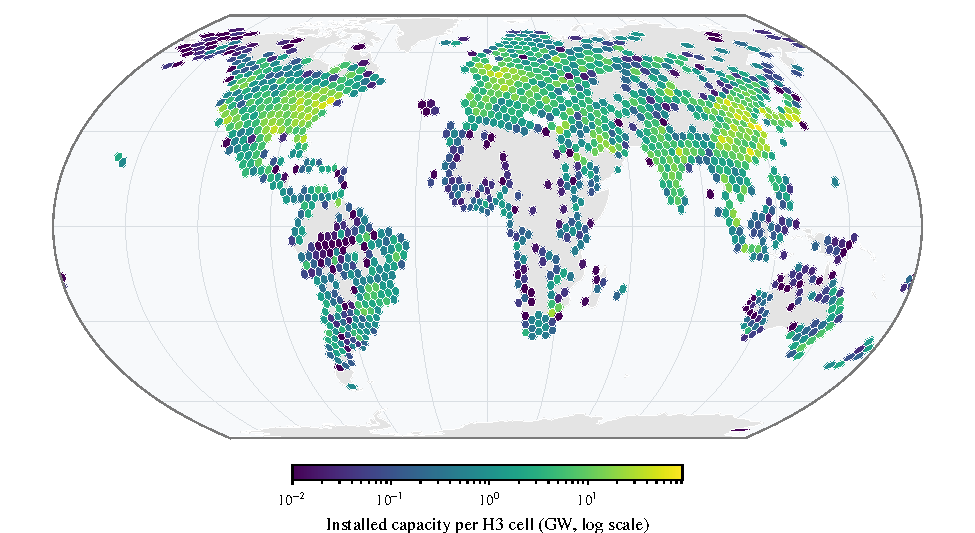
\includegraphics{figs/fig_global_map.pdf}
  \caption{Asset geography used in the simulation: installed capacity of the 34,936 plants in the Global Power Plant Database v1.3.0 \citep{byers2018gppd}, aggregated to H3 resolution-2 cells \citep{h3} (mean cell area about 87,000~km$^2$) and shown in the Equal Earth projection \citep{savric2019equal}. The simulation uses the 11,107 plants whose owners hold at least three plants.}
  \label{fig:globalmap}
\end{figure}





\subsection{E1: Geolocation precision versus hazard scale}
For each $\ell$ we draw 30 fields and compare exposures computed at true and degraded locations for seven error scales and for country-level geocoding. Figure~\ref{fig:master} plots asset-level Spearman correlations against $\sigma/\ell$. All 49 combinations of $\ell$ and $\sigma$ collapse onto the curve predicted by Proposition~\ref{prop:corr}, with a mean absolute deviation of 0.002. The largest deviation, 0.024, occurs at the longest correlation lengths, where assets are clustered relative to $\ell$ (the mean pairwise correlation $\bar c$ reaches 0.13 at $\ell = 1{,}000$~km); the finite-domain correction of Remark~\ref{rem:finite} reduces the mean deviation further to 0.0019.

\begin{figure}[t]
  \centering
  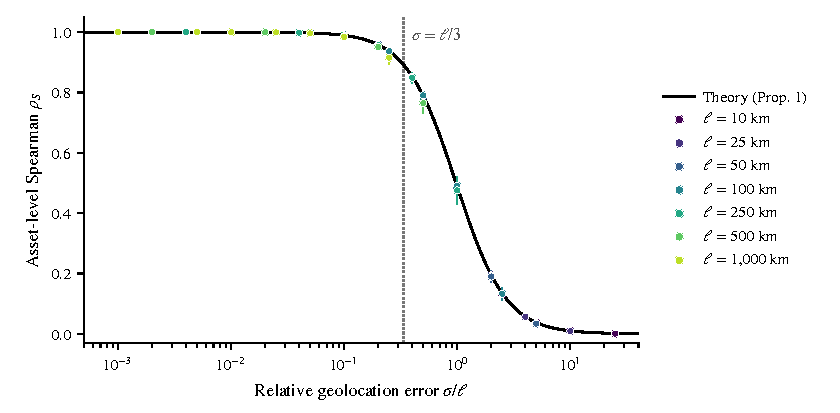
\includegraphics{figs/fig_master_curve.pdf}
  \caption{Asset-level fidelity of exposure under Gaussian geolocation error: Spearman correlation between hazard values at true and perturbed locations of 11,107 plants, plotted against $\sigma/\ell$ for seven correlation lengths and seven error scales (mean $\pm$ s.d.\ over 30 fields). The black curve is Equation~\eqref{eq:spearman}; the dotted line marks the design rule $\sigma = \ell/3$.}
  \label{fig:master}
\end{figure}

Firm-level fidelity (Figure~\ref{fig:heatmap}) is somewhat higher than asset-level fidelity at the same $\sigma/\ell$---between 0.53 and 0.63 at $\sigma = \ell$, compared with about 0.48---because averaging over a firm's assets dampens independent location errors. Two results stand out. First, country-level geocoding destroys most of the signal: firm-level rank correlations are at most 0.11 for $\ell \leq 100$~km and only 0.29--0.54 for $\ell$ between 250 and 1,000~km. Second, city-level geolocation ($\sigma = 25$~km) is adequate for regional hazards, with rank correlations of at least 0.99 for $\ell \geq 250$~km, but not for local ones (0.57 at $\ell = 25$~km).

\begin{figure}[t]
  \centering
  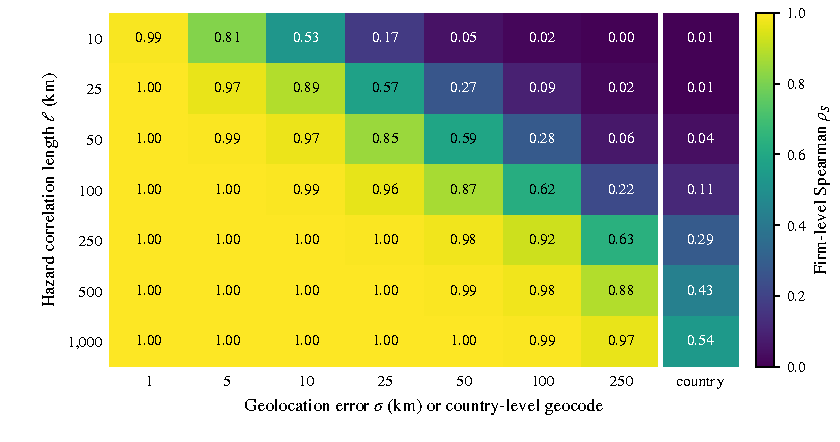
\includegraphics{figs/fig_firm_heatmap.pdf}
  \caption{Firm-level fidelity: Spearman correlation between capacity-weighted firm exposures computed at true and degraded locations (1,247 pseudo-firms; mean over 30 fields). The rightmost column replaces every asset's location by its country's label point.}
  \label{fig:heatmap}
\end{figure}

\subsection{E2: Extraction and geolocation errors in quadrant classification}
Figure~\ref{fig:accuracy} reports four-class quadrant accuracy, measured against quadrants computed from true exposure and true disclosure, for a local ($\ell = 25$~km) and a regional ($\ell = 500$~km) hazard. Extraction error reduces accuracy almost linearly, by about 2.75 percentage points per 0.1 increase in $\varepsilon$, for both hazards. The slope has a simple explanation: an adjacent-level error changes the quadrant only when it crosses $\tau_D$, which happens for levels 1 and 2 with probability $\varepsilon/2$ each, giving an expected loss of $\varepsilon(\pi_1 + \pi_2)/2 = 0.275\,\varepsilon$ for the level shares $\pi$ used here.

Geolocation error, in contrast, depends strongly on the hazard. For the local hazard, city-level error ($\sigma = 25$~km) alone reduces accuracy from 1.00 to 0.70, a loss more than five times larger than that from a 20\% extraction error rate (accuracy 0.945), and reduces the F1 score of the silent-risk class to 0.62; country-level geocoding brings accuracy down to 0.50. For the regional hazard, the same city-level error costs just over one percentage point (0.987), whereas country-level geocoding still costs about 36 points (0.635). The two error sources combine approximately additively; for the local hazard with $\sigma = 25$~km and $\varepsilon = 0.2$, accuracy is 0.666. The practical implication is a hazard-specific allocation of engineering effort: for local hazards, investment in geolocation dominates; for regional hazards, extraction quality matters more.

\begin{figure}[t]
  \centering
  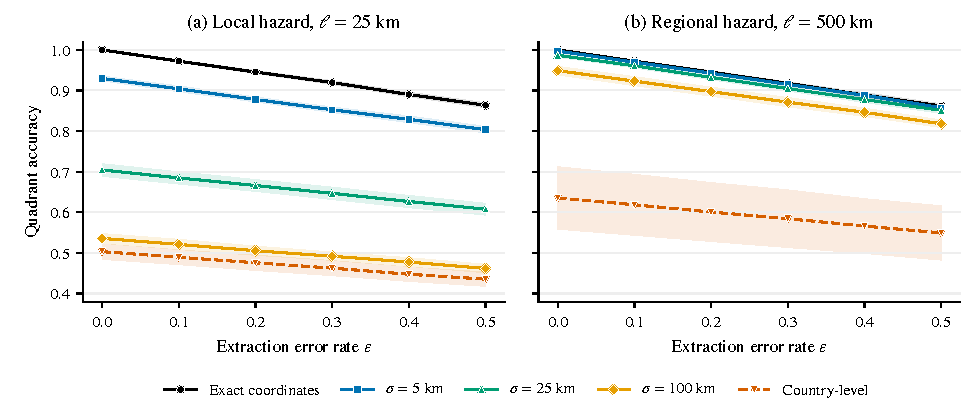
\includegraphics{figs/fig_quadrant_accuracy.pdf}
  \caption{Four-class quadrant accuracy as a function of the extraction error rate $\varepsilon$ for a local (a) and a regional (b) hazard, under exact, Gaussian-perturbed ($\sigma$ = 5, 25 and 100~km) and country-level asset locations. Lines show means and bands $\pm 1$ s.d.\ over 30 replications.}
  \label{fig:accuracy}
\end{figure}

\subsection{E3: Uncertainty propagation}
We next ask whether propagating uncertainty improves decisions. We fix a flood-like hazard ($\ell = 50$~km), city-level geolocation error ($\sigma = 25$~km), an extraction error rate of $\varepsilon = 0.25$, and hazard-model uncertainty represented by a five-member ensemble whose members correlate with the true field at $\sqrt{1-\kappa^2} \approx 0.92$. The predictive distribution $P(D \mid \hat D)$ is estimated on a simulated calibration sample of 500 annotated reports. We compare a point estimate, which uses the ensemble mean at the estimated locations and the extracted level, with three Monte Carlo variants that propagate extraction uncertainty only, location and hazard-model uncertainty only, or all three jointly. Silent-risk firms make up 16.1\% of firms on average.

\begin{table}[t]
\caption{Uncertainty propagation for identifying silent-risk firms (E3): means over 20 replications, standard deviations in parentheses. Brier scores and expected calibration error (ECE) evaluate $P(Q_i=\text{silent})$; AP is average precision. Precision, recall and the share of firms flagged refer to the point classification for the point estimate and to the rule $P(Q_i=\text{silent}) \geq 0.8$ for the Monte Carlo (MC) variants. Bold marks the best value in each probabilistic or precision column.}
\label{tab:e3}
\centering
\fontsize{8}{10}\selectfont
\setlength{\tabcolsep}{4.5pt}
\begin{tabular}{@{}lcccccc@{}}
\toprule
& \multicolumn{3}{c}{Probabilistic quality} & \multicolumn{3}{c}{Flagging silent-risk firms} \\
\cmidrule(lr){2-4}\cmidrule(l){5-7}
Method & Brier $\downarrow$ & ECE $\downarrow$ & AP $\uparrow$ & Precision $\uparrow$ & Recall & Flagged \\
\midrule
Point estimate & 0.100 (.008) & -- & -- & 0.676 (.029) & 0.728 (.038) & 17.4\% \\
MC: extraction only & 0.091 (.007) & 0.075 (.009) & 0.573 (.041) & 0.675 (.030) & 0.707 (.057) & 16.9\% \\
MC: location + hazard model & 0.075 (.005) & 0.047 (.007) & 0.712 (.032) & 0.803 (.038) & 0.429 (.034) & 8.6\% \\
MC: full propagation & \textbf{0.072} (.004) & \textbf{0.033} (.006) & \textbf{0.732} (.026) & \textbf{0.842} (.029) & 0.299 (.057) & 5.7\% \\
\bottomrule
\end{tabular}
\end{table}


Table~\ref{tab:e3} and Figure~\ref{fig:propagation} summarise the results. Full propagation gives the best probabilistic predictions: the Brier score falls from 0.100 for the point estimate to 0.072, and expected calibration error falls from 0.075 with extraction-only propagation to 0.033. Ignoring location and hazard-model uncertainty makes probabilities overconfident: firms to which extraction-only propagation assigns $P(\text{silent}) \geq 0.8$ are silent in only about 68\% of cases.

Propagation does not create information. At the point estimate's recall of 0.73, the propagated methods and the point estimate achieve essentially the same precision (0.67--0.68). What propagation adds is the ability to use the information selectively: the precision--recall curve of full propagation dominates that of extraction-only propagation, and a rule that flags a firm only when $P(\text{silent}) \geq 0.8$ attains a precision of 0.84, against 0.68 for the point estimate, while flagging 5.7\% of firms and recovering 30\% of silent-risk firms. Where a false finding of silence is costly, as in supervisory triage or public reporting, this abstention-based operating point is preferable to a point classification.

\begin{figure}[t]
  \centering
  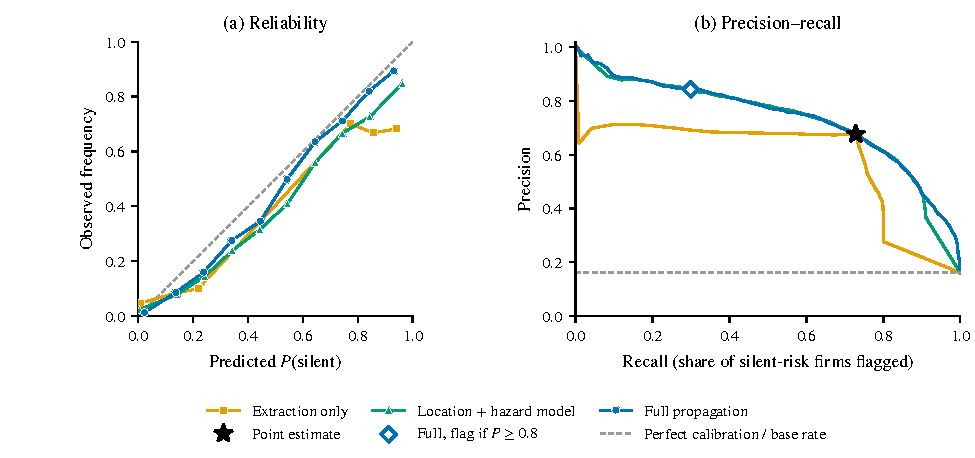
\includegraphics{figs/fig_propagation.pdf}
  \caption{Uncertainty propagation for identifying silent-risk firms ($\ell = 50$~km, $\sigma = 25$~km, $\varepsilon = 0.25$, five-member hazard ensemble; 20 replications pooled). (a)~Reliability of predicted probabilities, for bins containing at least 30 firms. (b)~Precision--recall curves; the star marks the point estimate and the diamond the rule that flags a firm when $P(\text{silent}) \geq 0.8$ under full propagation. The dashed line in (b) is the base rate of 16.1\%.}
  \label{fig:propagation}
\end{figure}

% =====================================================================
\section{Evaluation protocol for the empirical programme}
\label{sec:eval}

The simulation establishes how the DGI behaves when the error processes are known; the empirical programme must measure those processes. Table~\ref{tab:protocol} lists the evaluation of each component. Three design choices deserve emphasis. First, the gold standard is stratified by jurisdiction, language and sector, so that performance in under-represented markets is measured rather than assumed, and inter-annotator agreement on disclosure levels is reported with Krippendorff's $\alpha$ \citep{krippendorff2004content}. Second, geolocation error scales $\sigma_r$ are estimated against registries with known coordinates; Proposition~\ref{prop:corr} shows that these scales, relative to each hazard's correlation length, decide whether exposure estimates are informative at all. Third, exposure is computed from more than one hazard product, so that the disagreement documented by \citet{hain2022physical} becomes part of the reported uncertainty rather than a hidden modelling choice.

\begin{table}[t]
\caption{Evaluation protocol for the components of W2C.}
\label{tab:protocol}
\centering
\small
\begin{tabularx}{\textwidth}{@{}l>{\raggedright\arraybackslash}X>{\raggedright\arraybackslash}X@{}}
\toprule
Component & Reference data & Metrics \\
\midrule
Disclosure level $D$ & Double-annotated gold set, stratified by jurisdiction, language and sector & Macro-F1; quadratic-weighted $\kappa$; Krippendorff's $\alpha$ between annotators; ECE; conformal coverage and set size \\
Numeric metrics & XBRL facts (e.g., BRSR); CDP responses where licensed & Exact match; relative error $\leq 1\%$; accuracy of units, scope and boundary qualifiers \\
Provenance & Gold page and bounding box & Page accuracy; bounding-box intersection over union \\
Asset geolocation & Registry coordinates (GPPD, GEM, Climate TRACE) & Median error (km); share within 10 and 25~km; calibration of $\sigma_r$ \\
Hazard exposure & Several hazard products and ensemble members & Cross-product rank agreement \\
End to end & Expert review of a stratified sample of firms & Quadrant agreement; precision of silent-risk flags at fixed coverage \\
\bottomrule
\end{tabularx}
\end{table}

% =====================================================================
\section{Research agenda and identification strategies}
\label{sec:agenda}

W2C is designed to answer three empirical questions.
\begin{enumerate}[label=\textbf{RQ\arabic*.}, leftmargin=3.2em]
  \item \emph{Measurement.} How accurately can taxonomy-aligned disclosures and asset locations be extracted across languages and reporting regimes, and how much does distant supervision from XBRL improve performance in languages without labelled data?
  \item \emph{Description.} How large is the gap between disclosed and modelled physical risk, and how does it vary across hazards, sectors and countries? Quadrant probabilities aggregated on H3 cells provide the descriptive basis.
  \item \emph{Explanation and consequences.} Do mandatory disclosure regimes close the gap, and do markets price undisclosed exposure?
\end{enumerate}

For RQ3, the staggered adoption of ISSB-aligned requirements across jurisdictions provides variation in treatment timing that can be analysed with heterogeneity-robust difference-in-differences estimators \citep{callaway2021did}, with the firm-level DGI as outcome and firms in jurisdictions not yet treated as comparisons. Threats include anticipation, selection into early adoption and concurrent reforms; event-time plots and placebo outcomes address them in part. A complementary design exploits realised hazard events: when the footprint of a flood or cyclone intersects a firm's assets, an event study \citep{mackinlay1997event} can test whether abnormal returns differ between firms that had disclosed the exposure and firms classified as silent. Because the DGI is estimated with error, regressions should use its full posterior---through multiple imputation over Monte Carlo draws or errors-in-variables corrections \citep{carroll2006measurement}---rather than point estimates.

Thailand offers a natural deep-dive case. Listed Thai companies report through the Form 56-1 One Report in Thai and English, which tests multilingual extraction; power and industrial assets cluster in the Chao Phraya basin and along the Eastern Seaboard (Figure~\ref{fig:thailand}); and the 2011 floods, which disrupted manufacturing and global supply chains, provide a historical shock against which exposure estimates can be validated. Because the framework is global by design, lessons from the deep dive transfer to other markets with similar data constraints.

% =====================================================================
\section{Discussion}
\label{sec:discussion}

\paragraph{Limitations of the simulation.} The simulation abstracts from features of real data. Hazard fields are stationary and Gaussian, whereas real hazards are non-stationary and heavy-tailed; location errors are Gaussian, whereas geocoding errors are structured by administrative boundaries; and disclosure behaviour follows a stylised latent-awareness model. The asset sample comes from a single sector, and its owner field over-represents jurisdictions with open power-sector data, notably the United States. These choices make the ground truth known and the theory testable; they do not substitute for the empirical evaluation of Section~\ref{sec:eval}.

\paragraph{Exposure is not risk.} The DGI compares disclosure with modelled hazard exposure, not with vulnerability, adaptation or financial materiality; a firm whose assets in a flood plain are well protected may rationally disclose little. Asset weights should therefore reflect economic significance where it can be measured, and quadrant labels should be read as prompts for scrutiny rather than findings of non-compliance. Asset coverage is also incomplete: registries cover energy and heavy industry far better than services or agriculture, and firms' own location disclosures are uneven, which is itself an aspect of the gap that W2C measures.

\paragraph{Ethics and responsible use.} Labelling a firm as silent risk has reputational consequences. W2C therefore reports probabilities rather than labels, abstains below a confidence threshold, exposes provenance so that any classification can be checked against its sources, and should give firms a channel to correct errors. Language models used for extraction can produce plausible but wrong values; verification, provenance and calibration are the safeguards, and no value enters the published dataset without a source location. Source reports are publicly available but protected by copyright, so W2C publishes extracted facts, hashes and links rather than documents; some hazard and biodiversity datasets restrict commercial use, which constrains the redistribution of derived products.

\paragraph{Environmental footprint.} Processing tens of thousands of reports with large models consumes energy \citep{strubell2019energy}. W2C reserves large models for teacher labelling and validation and uses distilled models for bulk processing, and we recommend reporting the computational footprint of the pipeline \citep{lacoste2019quantifying}---a modest but consistent requirement for research that evaluates other organisations' climate disclosures.

% =====================================================================
\section{Conclusion}
\label{sec:conclusion}

Climate disclosure is becoming abundant, standardised and consequential, but its connection to the physical world remains largely unmeasured. Words to Coordinates links what firms disclose to what their assets face, carrying provenance and uncertainty from source documents to a peer-relative Disclosure Gap Index and a global map. Our analysis yields a simple, testable design rule---geolocation error should be at most one third of a hazard's correlation length---and shows, on real asset geography, that country-level location information is inadequate for physical risk assessment, that geolocation rather than extraction is the binding constraint for local hazards, and that propagating uncertainty turns noisy measurements into calibrated, decision-ready probabilities. The next step is the empirical programme set out in Sections~\ref{sec:eval} and~\ref{sec:agenda}: building the multilingual benchmark, estimating real error scales and measuring the disclosure gap across the world's markets. Because location is also the first step of nature-related assessment under the TNFD's approach \citep{tnfd2023}, the same architecture extends naturally from climate to nature.

\section*{Data and code availability}
The simulation uses the Global Power Plant Database v1.3.0 (CC BY 4.0) \citep{byers2018gppd} and Natural Earth boundaries (public domain) \citep{naturalearth2024}. All other inputs are simulated with fixed random seeds. Code to reproduce every result and figure is available from the author on request.

\section*{Use of AI tools}
Generative AI tools were used to assist with drafting text, writing code and preparing figures. The author reviewed the manuscript and takes full responsibility for its content.

\bibliographystyle{plainnat}
\bibliography{references}

% =====================================================================
\appendix
\section{Proof of Proposition~\ref{prop:corr} and Remark~\ref{rem:finite}}
\label{app:proof}

\paragraph{Pearson correlation.} Conditional on $\bm\delta$, stationarity and isotropy imply that $\big(Z(\x), Z(\x + \bm\delta)\big)$ is bivariate normal with unit variances and correlation $\rho(\|\bm\delta\|)$. Because $\bm\delta$ is independent of the field, $\operatorname{Cov}\big(Z(\x), Z(\hat\x)\big) = \E_{\bm\delta}\big[\rho(\|\bm\delta\|)\big]$, and both marginal variances equal one. With $\bm\delta\sim\mathcal{N}(\mathbf{0},\sigma^2 I_2)$, $\|\bm\delta\|^2/\sigma^2 \sim \chi^2_2$, so that $T := \|\bm\delta\|^2/(2\sigma^2)$ is standard exponential and $\rho(\|\bm\delta\|) = \exp\{-(\sigma^2/\ell^2)\,T\}$. Hence
\[
  \E\big[\rho(\|\bm\delta\|)\big] = \int_0^\infty e^{-(\sigma^2/\ell^2) t}\, e^{-t}\, dt = \frac{1}{1 + \sigma^2/\ell^2} = \frac{\ell^2}{\ell^2 + \sigma^2},
\]
which proves \eqref{eq:pearson}.

\paragraph{Spearman correlation.} Spearman's correlation is invariant under strictly increasing transformations, so we may take $g$ to be the identity. For a pair $(X, Y)$ with continuous marginals, the population Spearman correlation is $\rho_S = 3\big[P\{(X_1 - X_2)(Y_1 - Y_3) > 0\} - P\{(X_1 - X_2)(Y_1 - Y_3) < 0\}\big]$, where $(X_j, Y_j)$, $j = 1, 2, 3$, are independent copies of $(X, Y)$. Here $X = Z(\x_a)$ and $Y = Z(\hat\x_a)$, and independent copies correspond to independent assets. The marginals of $X$ and $Y$ are standard normal whatever the value of $\bm\delta$, so $X_2$ and $Y_3$ are independent standard normal variables. Conditional on the displacement $\bm\delta_1$ of the first copy, $(X_1, Y_1)$ is bivariate normal with correlation $\rho(\|\bm\delta_1\|)$, and the bracket equals the bivariate-normal value $(6/\pi)\arcsin\{\rho(\|\bm\delta_1\|)/2\}$. The expression is linear in the distribution of $(X_1, Y_1)$, so averaging over $\bm\delta_1$, with the substitution above, gives \eqref{eq:spearman}. Both \eqref{eq:pearson} and \eqref{eq:spearman} depend on $(\sigma, \ell)$ only through $\sigma/\ell$. \hfill$\square$

\paragraph{Finite domain.} For $n$ assets observed in a single realisation of the field, the expected within-sample covariance between $Z(\x_a)$ and $Z(\hat\x_a)$ is approximately $\rho - \bar c$, and the expected within-sample variance of $Z(\x_a)$ is approximately $1 - \bar c$, where $\bar c = n^{-2}\sum_{a,b}\rho(d_{ab})$ is the mean pairwise correlation and the approximation neglects terms of order $1/n$ and differences between $\rho(d_{ab})$ and $\rho(\|\x_a - \hat\x_b\|)$. The within-sample correlation is therefore approximately $(\rho - \bar c)/(1 - \bar c)$. For the plant sample, $\bar c$ ranges from 0.0004 at $\ell = 10$~km to 0.13 at $\ell = 1{,}000$~km.

\section{Simulation details}
\label{app:sim}

\paragraph{Random fields.} Hazard fields are generated as
\[
  Z(\x) = \sqrt{2/J}\, \sum_{j=1}^{J} \cos\big(\bm\omega_j^\top \mathbf{p}(\x) + b_j\big), \qquad \bm\omega_j \sim \mathcal{N}(\mathbf{0}, \ell^{-2} I_3), \quad b_j \sim \mathrm{Uniform}[0, 2\pi),
\]
where $\mathbf{p}(\x)\in\mathbb{R}^3$ is the Earth-centred Cartesian position, in kilometres, of $\x$ on a sphere of radius 6,371~km, and $J = 1{,}024$. As $J\to\infty$, $Z$ converges to a Gaussian process with covariance $\exp\{-\|\mathbf{p}(\x) - \mathbf{p}(\x')\|^2/(2\ell^2)\}$ \citep{rahimi2007random}. Restricted to the sphere, this is a valid covariance in chordal distance, which is approximately equal to great-circle distance at the scales considered.

\paragraph{Location errors.} Gaussian perturbations are applied in the local tangent plane, converting kilometres to degrees of latitude and longitude at each asset's latitude. Country-level geocoding uses the Natural Earth label point of the asset's country; for the single country code in the database without a match, the mean location of that country's plants is used.

\paragraph{Ensemble members.} Hazard-model members are $Z^{(m)} = \sqrt{1-\kappa^2}\,Z + \kappa\,\eta_m$, where the $\eta_m$ are independent fields with the same correlation length as $Z$. The point estimate uses the ensemble mean.

\begin{table}[h]
\caption{Parameters of the simulation study. E1--E3 denote the three experiments.}
\label{tab:params}
\centering
\small
\begin{tabularx}{\textwidth}{@{}l>{\raggedright\arraybackslash}X@{}}
\toprule
Component & Setting \\
\midrule
Assets & GPPD v1.3.0; 11,107 plants of 1,247 owners with $\geq 3$ plants, 76 countries; $w_a$ = capacity share \\
Hazard fields & Gaussian random fields, squared-exponential kernel, 1,024 random Fourier features; $g = \Phi$ \\
Correlation length $\ell$ (km) & E1: 10, 25, 50, 100, 250, 500, 1,000; \; E2: 25, 500; \; E3: 50 \\
Geolocation error $\sigma$ (km) & E1: 1, 5, 10, 25, 50, 100, 250, country level; \; E2: 0, 5, 25, 100, country level; \; E3: 25 \\
Disclosure model & $\beta = 0.4$; level shares $(0.15, 0.30, 0.25, 0.20, 0.10)$ \\
Extraction error $\varepsilon$ & E2: 0, 0.1, \ldots, 0.5; \; E3: 0.25 \\
Quadrant thresholds & $\tau_E = 0.5$, $\tau_D = 2$ \\
Hazard-model ensemble & E3: $M = 5$ members, $Z^{(m)} = \sqrt{1-\kappa^2}\,Z + \kappa\,\eta_m$ with $\kappa = 0.4$ \\
Calibration of $P(D\mid\hat D)$ & E3: 500 simulated annotated reports, add-one smoothing \\
Monte Carlo & E3: $K = 80$ draws \\
Replications & E1: 30 fields per $\ell$; \; E2: 30 per $\ell$, three extraction draws each; \; E3: 20 \\
\bottomrule
\end{tabularx}
\end{table}

\paragraph{Reproducibility.} Each experimental unit (a correlation length in E1 and E2, a replication in E3) uses its own random-number stream derived from a fixed master seed, so results do not depend on the order or partitioning of computation. Evaluation metrics follow standard definitions: expected calibration error uses ten equal-width bins, and average precision is computed with scikit-learn.

\end{document}
